\documentclass{winnower}
\usepackage{indentfirst}
\usepackage{graphicx}
\usepackage{caption}
\usepackage{subfigure}
\usepackage{xcolor}
\usepackage{float}
\usepackage[section]{placeins}
\usepackage{multirow}
\usepackage{booktabs}
\setlength{\belowcaptionskip}{-0.5cm}

\begin{document}

\title{Homework5 report}

\author{Haoyu Guan}

\affil[1]{Questrom School of Business, Boston University}







\date{2020.02.11}

\maketitle




%-------------------------------------------------%
\section{Implementation of Breeden-Litzenberger}
%-------------------------------------------------%


\indent You are given the following volatility data:

%\vspace{12 pt}
$$
\begin{array}{|l|c|r|}
\hline \text { Expiry / Strike } & 1 \mathrm{M} & 3 \mathrm{M} \\
\hline 10 \mathrm{DP} & 32.25 \% & 28.36 \% \\
\hline 25 \mathrm{DP} & 24.73 \% & 21.78 \% \\
\hline 40 \mathrm{DP} & 20.21 \% & 18.18 \% \\
\hline 50 \mathrm{D} & 18.24 \% & 16.45 \% \\
\hline 40 \mathrm{DC} & 15.74 \% & 14.62 \% \\
\hline 25 \mathrm{DC} & 13.70 \% & 12.56 \% \\
\hline 10 \mathrm{DC} & 11.48 \% & 10.94 \% \\
\hline
\end{array}
$$


You also know that the current stock price is 100, the risk-free rate is 0, and the asset
pays no dividends.

NOTE: The table of strikes is quoted in terms of Deltas, where the DP rows indicate "X
Delta Puts" and the DC rows indicate "X Delta Calls".




\textbf{(a) Using the table of quoted (Black-Scholes) Deltas and volatilities, extract a table of
strikes corresponding to each option.}

$$
\begin{array}{|l|c|r|}
\hline \text { Expiry / Strike } & 1 \mathrm{M} & 3 \mathrm{M} \\
\hline 10 \mathrm{DP} & 89.138758  & 84.225674  \\
\hline 25 \mathrm{DP} & 95.542103  & 93.470685  \\
\hline 40 \mathrm{DP} & 98.700642  & 98.127960  \\
\hline 50 \mathrm{D} & 100.138720  & 100.338826  \\
\hline 40 \mathrm{DC} & 101.262273  & 102.141761  \\
\hline 25 \mathrm{DC} & 102.783751  & 104.532713  \\
\hline 10 \mathrm{DC} & 104.395838  & 107.422225  \\
\hline
\end{array}
$$

\textbf{(b) Choose an interpolation scheme that defines the volatility function for all strikes, $\sigma(K)$}

We use linear regression to generate interpolation of $\sigma(K)$
$$\sigma(K)_{1M}=-0.01379K+1.55779$$

$$\sigma(K)_{3M}=-0.00767K+0.93223$$



\newpage

\textbf{(c) Extract the risk neutral density for 1 \& 3 month options. Comment on the differences
between the two distributions. Is it what you would expect?}

\begin{figure*}[!h]
\begin{center}
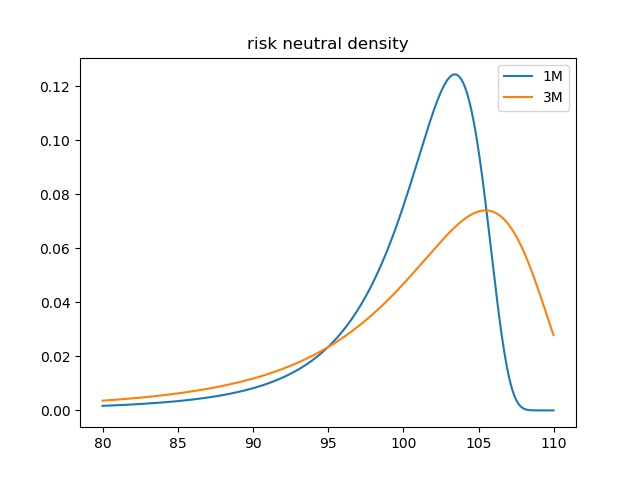
\includegraphics[scale=0.6]{1_1.jpg}
\caption
{risk neutral density}
\label{fig:f1}
\end{center}
\end{figure*}

\textbf{(d) Extract the risk neutral density for 1 \& 3 month options using a constant volatility
equal to the 50D volatility. Contrast these densities to the densities obtained above.}

\begin{figure*}[!h]
\begin{center}
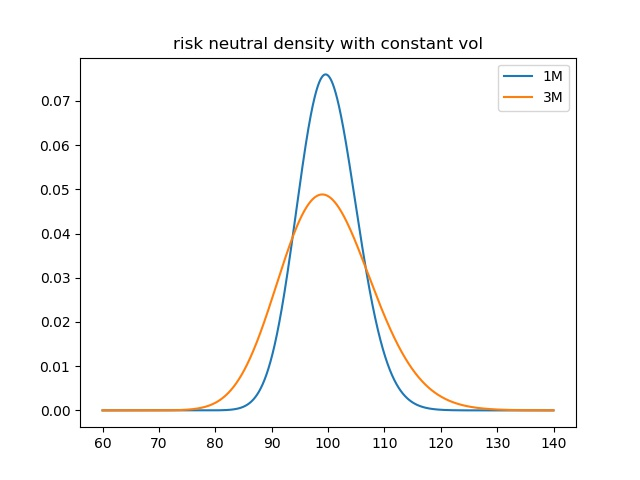
\includegraphics[scale=0.6]{1_2.jpg}
\caption
{risk neutral density with constant vol}
\label{fig:f1}
\end{center}
\end{figure*}

\textbf{(e) Price the following European Options using the densities you constructed in (1c).}
\\


i. 1M European Digital Put Option with Strike 110.

$$P_{1M,K=110}^{put}=0.943151020771406$$

ii. 3M European Digital Call Option with Strike 105.

$$P_{3M,K=105}^{call}=0.32706708056889877$$

iii. 2M European Call Option with Strike 100.

$$P_{2M,K=100}^{call}=1.3364446175053875$$

\section{Calibration of Heston Model}

\indent Recall that the Heston Model is defined by the following system of SDE��s:

$$
\begin{aligned}
d S_{t} &=r S_{t} d t+\sqrt{\nu_{t}} S_{t} d W_{t}^{1} \\
d \nu_{t} &=\kappa\left(\theta-\nu_{t}\right) d t+\sigma \sqrt{\nu_{t}} d W_{t}^{2} \\
\operatorname{Cov}\left(d W_{t}^{1}, d W_{t}^{2}\right) &=\rho d t
\end{aligned}
$$

Recall also that the characteristic function for the Heston Model is known to be:

$$
\begin{aligned}
\omega(u) &=\frac{\exp \left(i u \ln S_{0}+i u(r-q) t+\sigma^{-2}\{\kappa \theta t(\kappa-i \rho \sigma u)\}\right)}{\left(\cosh \frac{\lambda t}{2}+\frac{\kappa-i \rho \sigma u}{\lambda} \sinh \frac{\lambda t}{2}\right)^{\frac{2 \pi \theta}{\partial^{2}}}} \\
\Phi(u) &=\omega(u) \exp \left(\frac{-\left(u^{2}+i u\right) \nu_{0}}{\lambda \operatorname{coth} \frac{\lambda t}{2}+\kappa-i \rho \sigma u}\right) \\
\lambda &=\sqrt{\sigma^{2}\left(u^{2}+i u\right)+(\kappa-i \rho \sigma u)^{2}}
\end{aligned}
$$


See the attached spreadsheet for options data.$r=1.5 \%, q=1.77 \%, S_{0}=267.15$

Consider the given market prices and the following equal weight least squares minimization function:

$$
\vec{p}_{\min }=\min _{\vec{p}}\left\{\sum_{\tau, K}\left(\tilde{c}(\tau, K, \vec{p})-c_{\tau, K}\right)^{2}\right\}
$$

where $\tilde{c}(\tau, K, \vec{p})$ is the FFT based model price of a call option with expiry $\tau$ and strike $K$.


\textbf{(a) Check the option prices for arbitrage. Are there arbitrage opportunities at the mid?
How about after accounting for the bid-ask spread? Remove any arbitrage violations
from the data}
\\

We must make sure it is no increasing or no decreasing for the bid price and ask price. We find there is no arbitrage opportunities at the mid.
\\

\textbf{(b) Using the FFT Pricing code from your last homework, find the values of $\kappa, \theta, \sigma, \rho$ and $\nu_{0}$ that minimize the equal weight least squared pricing error. You may choose the starting point and upper and lower bounds of the optimization. You may also choose whether to calibrate to calls, puts, or some combination of the two.}

NOTE: In $R$, the optima function can be used to perform this optimization, which has a parameter named method which can be set to Nelder-Mead.

Note also that you are given data for multiple expiries, each of which should use the same parameter set, but will require a separate call to the $F F T$ algorithm.
\\

The values of $\kappa, \theta, \sigma, \rho$ and $\nu_{0}$ that minimize the equal weight least squared pricing error is

$$\kappa=2.00994809$$
$$\theta=0.2297692$$
$$\sigma=0.49121625$$
$$\rho=-0.98452449$$
$$\nu_{0}=0.09823346$$

The bounds are  

$$\kappa\in(0.01,5)$$
$$\theta\in(0,2)$$
$$\sigma\in(0,1)$$
$$\rho\in(-1,1)$$
$$\nu_{0}\in(0,1)$$
\\

\textbf{(c) Try several starting points and several values for the upper and lower bounds of your
parameters. Does the optimal set of parameters change? If so, what does this tell you
about the stability of your calibration algorithm?}
\\

I set start point at [2,0.2,0.5,-1,0.1]. And change the bound to

$$\kappa\in(0.01,2.5)$$
$$\theta\in(0,1)$$
$$\sigma\in(0,1)$$
$$\rho\in(-1,0.5)$$
$$\nu_{0}\in(0,0.5)$$

The values of $\kappa, \theta, \sigma, \rho$ and $\nu_{0}$ that minimize the equal weight least squared pricing error is

$$\kappa=2.21974776$$
$$\theta=0.20018674$$
$$\sigma=0.24647732$$
$$\rho=-0.9394907$$
$$\nu_{0}=0.03040164$$

The value will be changed
\\

\textbf{(d) Instead of applying an equal weight to each option consider the following function which makes the weights inversely proportional to the quoted bid-ask spread:}

$$
\begin{aligned}
\omega_{\tau, K} &=\frac{1}{c_{\tau, K, \text { ask }}-c_{\tau, K, \text { bid }}} \\
\vec{p}_{\min } &=\min _{\vec{p}}\left\{\sum_{\tau, K}\left(\omega_{\tau, K} \tilde{c}(\tau, K, \vec{p})-c_{\tau, K}\right)^{2}\right\}
\end{aligned}
$$

where as before $\tilde{c}(\tau, K, \vec{p})$ is the FFT based model price of a call option with expiry
$\tau,$ strike $K .$ Repeat the calibration with this objective function and comment on how this weighting affects the optimal parameters.
\\

I set start point at [2,0.2,0.5,-1,0.1]. And change the bound to

$$\kappa\in(0.01,2.5)$$
$$\theta\in(0,1)$$
$$\sigma\in(0,1)$$
$$\rho\in(-1,0.5)$$
$$\nu_{0}\in(0,0.5)$$

The values of $\kappa, \theta, \sigma, \rho$ and $\nu_{0}$ that minimize the equal weight least squared pricing error is

$$\kappa=2.5$$
$$\theta=5.17619099e-04$$
$$\sigma=9.04434986e-03$$
$$\rho=-9.99775028e-01$$
$$\nu_{0}=1.12893003e-04$$

The value will be changed a lot
\\



\section{Hedging Under Heston Model}

Consider a 3 month European call with strike 275 on the same underlying asset.

\textbf{(a) Calculate this option's Heston delta using finite differences. That is, calculate a first order central difference by shifting the asset price, leaving all other parameters constant and re-calculating the FFT based Heston model price at each value of $S_{0}$.}
\\

i. Compare this delta to the delta for this option in the Black-Scholes model. Are they different, and if so why? If they are different, which do you think is better and why? Which would you use for hedging?
\\

$$\Delta_{Heston}=0.4761809756138795$$
$$\Delta_{BS model}=0.36685871212686977$$

There are some differences between this two $\Delta$. I think the $\Delta_{Heston}$ is better because the model is more complex and suitable for hedging.
\\

ii. How many shares of the asset do you need to ensure that a portfolio that is long one unit of the call and short $x$ units of the underlying is delta neutral?
\\

Of course, answer is $\Delta$ shares of the asset could make it delta neutral.
\\

\textbf{(b) Calculate the vega of this option numerically via the following steps:}
\\

i. Calculate the Heston vega using finite differences. To do this, shift $\theta$ and $\nu_{0}$ by the same amount and calculate a first order central difference leaving all other parameters constant and re-calculating the FFT based Heston model price at each value of $\theta$ and $\nu_{0}$

$$\nu_{Heston}=131.8189035082184$$

ii. Compare this vega to the vega for this option in the Black-Scholes model. Are they different, and if so why?

$$\nu_{BS model}=50.2927918023669$$

There are some differences. Totally because of the model differences.









\end{document}
